\chapter{Planare Graphen}

\section{Polygone}

\begin{definition}[Liniensegment]
    Seien $ p, q \in \reals^2 $.
    Dann ist $ \{ p + \lambda (q - p) \mid \lambda \in [0, 1] \} $ ein \textit{Liniensegment}.
\end{definition}

\begin{definition}[Polygonzug]
    Sei $ P \subsetneq \reals^2 $.
    $ P $ ist ein Polygonzug, falss es eine Vereinigung von endlich vielen Liniensegmente ist und eine homöomorphische, d.h. bijektive und stetige, Abbildung von $ P $ zur Einheitsstrecke existiert.
\end{definition}

\begin{definition}[Polygon]
    Sei $ P \subsetneq \reals^2 $.
    $ P $ ist Polygon, falls es eine Vereinigung von endlich vielen Liniensegmenten ist und eine homöomorphische, d.h. bijektive und stetige, Abbildung von $ P $ zum Einheitskreis existiert.
\end{definition}

\begin{theorem}
    Sei $ P $ ein Polygon.
    Dann hat $ \reals^2 \setminus P $ zwei Regionen; innen und außen.
\end{theorem}

\section{Graphen in der Ebene}

\begin{definition}[Graph in der Ebene]
    Ein Graph $ G = (V, E) $ ist ein Graph in der Ebene, falls:
    \begin{enumerate}
        \item $ V \subsetneq \reals^2 $,
        \item $ e \in E $ ist ein Polygonzug,
        \item keine zwei Kanten haben zwei gleiche Endpunkte und
        \item für $ e_1, e_2 \in E $ gilt $ (e_1 \cap e_2) \setminus V = \emptyset $, d.h. bis auf die Endpunkte, schneiden sich Kanten nicht.
    \end{enumerate}
\end{definition}

\begin{definition}[Planar]
    Ein Graph $ G $ ist planar, falls er sich als Graph in der Ebene darstellen lässt.
\end{definition}

\begin{definition}[Facette/Face]
    Sei $ G = (V, E) $ ein Graph in der Ebene.
    Eine Region in $ \reals^2 \setminus \bigcup E $ ist eine \textit{Facette}/ein \textit{Face}.
    Die Facette, die außerhalb von $ G $ liegt ist die \textit{äußere Facette}; alle anderen sind \textit{innere Facetten}.
\end{definition}

\begin{theorem}[Eulersche Formel]
    Sei $ G $ ein verbundener Graph in der Ebene mit $ n $ Knoten, $ m $ Kanten und $ l $ Facetten.
    Dann gilt:
    \begin{equation*}
        n - m + l = 2
    \end{equation*}
\end{theorem}

\begin{proof}
    Sei $ n $ fixiert.
    Beweis per Induktion über $ m $.
    \begin{description}
        \item[IA] Sei $ m = n - 1 $\footnote{%
            Für $ m < n - 1 $ ist $ G $ nicht verbunden, d.h. die Eulersche Formel findet keine Anwendung.
        }.
        Dann ist $ G $ ein Baum und Bäume haben eine Facette, also:
        \begin{equation*}
            n - (n - 1) + 1 = n - n + 1 + 1 = 2
        \end{equation*}
        \item[IV] Es gelte $ n - m + l = 2 $.
        \item[IS] Zu zeigen ist, $ n - (m + 1) + l' = 2 $.
        Es kann angenommen werden, dass $ m \geq n $.
        Somit ist $ G $ kein Baum und damit ex. ein Kreis in $ G $.
        Sei $ e \in E $ eine Kante auf einem Kreis.
        $ e $ liegt damit auf der Grenze zweier Facetten $ f_1 $, $ f_2 $.

        Sei $ G' = G \setminus \{ e \} $.
        Dann ex. eine Facette $ f_e $ von $ G' $, die $ f_1 $ und $ f_2 $ enthält.
        $ G' $ hat also eine Kante und damit eine Facette weniger als $ G $.
        Somit gilt nach IV:
        \begin{align*}
            n - (m + 1) + l' &= n - (m + 1) + (l + 1) \\
            &= n - m - 1 + l + 1 \\
            &= n - m + l = 2
        \end{align*}
    \end{description}
\end{proof}

\begin{corollary}
    \label{cor:max-edges}
    Sei $ G = (V, E) $ ein Graph in der Ebene mit $ |V| \geq 3 $.
    $ G $ hat dann maximal $ 3n - 6 $ Kanten.
\end{corollary}

\section{Unterteilung von Graphen}

\begin{definition}[Unterteilung]
    Sei $ G = (V, E) $ ein Graph und $ e = \{ x, y \} \in E $.
    $ G' = (V \cup \{ w \}, E \setminus e \cup \{ \{ x, w \}, \{ w, y \} \}) $ ist eine Unterteilung von $ G $.
\end{definition}

\begin{definition}[Graph-Mimor/Subdivision]
    Ein Graph $ H $ ist ein Mimor von $ G = (V, E) $, falls:
    \begin{itemize}
        \item $ H $ durch Löscher einer Kante entstanden ist, d.h. $ H = G \setminus \{ e \} $ für ein $ e \in E $,
        \item $ H $ durch Löschen eines Knoten entstanden ist, d.h. $ H = G \setminus \{ v \} $ für ein $ v \in V $, oder
        \item $ H $ durch Kontraktion einer Kante entstanden ist, d.h. für eine Kante $ e = \{ x, y \} \in E $ ist $ H = (V \cup \{ w \}, E \setminus \{ e \} \cup \{ \{ a, w \} \mid \{ a, x \} \in E \lor \{ a, y \} \in E \}) $.
    \end{itemize}
\end{definition}

\begin{definition}
    Es seien:
    \begin{itemize}
        \item $ K_{3,3} = (\{ 1, \dots, 6 \}, \{ \{ i, j \} \mid i \mod 2 \ne j \mod 2 \})$
        \item $ K_5 = (\{ 1, \dots, 5 \}, \{ \{ i, j \} \mid 1 \leq i, j \leq 5 \}) $
    \end{itemize}
\end{definition}

\begin{remark}
    $ K_{3,3} $ ist der bis auf Isomorphismus eindeutig bestimmte bipartite Graph mit sechs Knoten.

    $ K_5 $ ist der vollständig verbundene Graph mit fünf Knoten.
\end{remark}

\begin{lemma}
    \label{lem:k33-planar}
    $ K_{3,3} $ ist nicht planar.
\end{lemma}

\begin{proof}
    Angenommen $ K_{3,3} $ ist planar.
    Dann ex. eine Einbettung in die Ebene.
    Da $ K_{3,3} $ bipartit ist, ex. kein Kreis mit 3 oder weniger Kanten in $ K_{3,3} $.
    Somit ist jede Facette der Einbettung von mindestens vier Kanten umgeben.
    Des Weiteren begrenzt jede Kante zwei Facetten.

    Sei $ n $ die Anzahl der Knoten, $ m $ die Anzahl der Kanten und $ l $ die Anzahl der Facetten der Einbettung in die Ebene von $ K_{3,3} $.
    Es gilt dann:
    \begin{equation*}
        l \leq \frac{2m}{4} = \frac{m}{2} = 3,5
    \end{equation*}

    Nach der Eulerschen Formel gilt jedoch ebenso:
    \begin{equation*}
        2 = n - m + l \leq 6 - 9 + 3,5 = 1,5
    \end{equation*}

    Widerspruch.
    Also ist $ K_{3,3} $ nicht planar.
\end{proof}

\begin{lemma}
    \label{lem:k5-planar}
    $ K_5 $ ist nicht planar.
\end{lemma}

\begin{remark}
    Hier ohne Beweis, jedoch auch kann auch für $ K_5 $ eine Ungleichung über die Eulersche Formel zum Widerspruch geführt werden.
\end{remark}

\begin{theorem}[Kuratowskis Theorem]
    Sei $ G $ ein Graph.
    $ G $ ist nicht planar gdw. weder $ K_{3,3} $ noch $ K_5 $ ist ein Mimor von $ G $.
\end{theorem}

\begin{proof}~\par
    \begin{description}
        \item[``($ \Leftarrow $)''] Dies folgt mehr oder weniger direkt aus den Lemmata \ref{lem:k33-planar} und \ref{lem:k5-planar}.
        \item[``($ \Rightarrow $)''] Angenommen $ G $ ist nicht planar, aber enthält weder $ K_{3,3} $ noch $ K_5 $ als Mimor.
        Wähle $ G $ minimal mit obigen Eigenschaften.

        Es gilt: $ G $ ist zwei verbunden.
        Ein Graph ist planar gdw. alle seine Blöcke sind planar.
        Angenommen, $ G $ wäre nicht zwei verbunden, dann enthält $ G $ einen nicht-planaren Block.
        Dies wäre ein Widerspruch zur Minimalität von $ G $.

        Es gilt: Kein Knoten in $ G $ hat Grad zwei.
        Sei $ v \in V $ mit $ \deg(v) = 2 $.
        Seien $ u, w \in V $ die Nachbarn von $ v $.
        Angenommen, $ \{ u, w \} \in E $. Dann bilden die Knoten $ \{ u, v, w \} $ einen planaren Subgraphen in $ G $.
        Widerspruch zur Minimalität von $ G $.
        Angenommen, $ \{ u, w \} \notin E $.
        Da $ G $ 2-verbunden ist, müssen weitere Pfade zwischen $ u $ und $ w $ existieren.
        Dann können diese Pfade sukzessive entfernt werden und $ \{ u, v\} $, $ \{ w, v \} $ kontraktiert.
        Dann ist $ G $ nicht mehr 2-verbunden und besteht aus zwei Blöcken.
        Widerspruch zur Minimalität von $ G $.

        Es gilt: Es ex. Kante $ e = \{ u, v \} \in E $ mit $ H = G \setminus \{ e \} $ ist 2-verbunden, d.h. es gibt einen Kreis $ C $, der $ u $ und $ v $ abdeckt, aber nicht $ e $ enthält. (Hier ohne Beweis.)

        Da $ G $ minimal gewählt, sodass $ G $ nicht planar, muss $ H $ planar sein.
        Bette $ H $ derart in die Ebene ein, dass gilt:
        \begin{itemize}
            \item Die Anzahl der Regionen innerhalb $ C $ sei maximal und
            \item falls es einen Kreis $ C' $ mit $ e \in C' $ gibt, dann hat $ C' $ höchstens so viele Facetten wie $ C $.
        \end{itemize}

        Sei $ C = u v_1 v_2 \dots v_{k-1} v v_{k + 1} \dots v_l, u $.
        Da die Einbettung so gewählt wurde, dass maximal Facetten in $ C $ liegen, kann es keinen Pfad mit Endpunkten in $ C $ außerhalb zu $ C $ geben.

        Es muss ebenso einen Pfad $ Q $ geben, der Knoten aus $ \{ v_1, \dots, v_{k - 1} \} $ und aus $ \{ v_{k + 1}, \dots, v_l \} $ verbindet und der außerhalb von $ C $ liegt.
        Ansonsten könnte die Kante $ \{ u, v \} $ außerhalb des Graphen gezeichnet werden, sodass $ G $ planar ist.

        Betrachte nun die Graphen in Abbildung \ref{fig:kuratowski-bsp}.
        Diese stellen alle Möglichkeiten dar, wie $ C $ aufgebaut sein kann.
        In diesen Abbildungen sieht man, dass Graphen \subref{fig:kuratowski-bsp1}-\subref{fig:kuratowski-bsp3} entsprechend der markierten Färbung und nach Löschen der rot-markierten Knoten/Kanten $ K_{3,3} $ einbetten.
        Graph \subref{fig:kuratowski-bsp4} bettet $ K_5 $ ein.
        Widerspruch zur Annahme.
    \end{description}

    \begin{figure}
        \centering
        \def\w{0.45\textwidth}
        \begin{subfigure}[c]{\w}
            \centering
            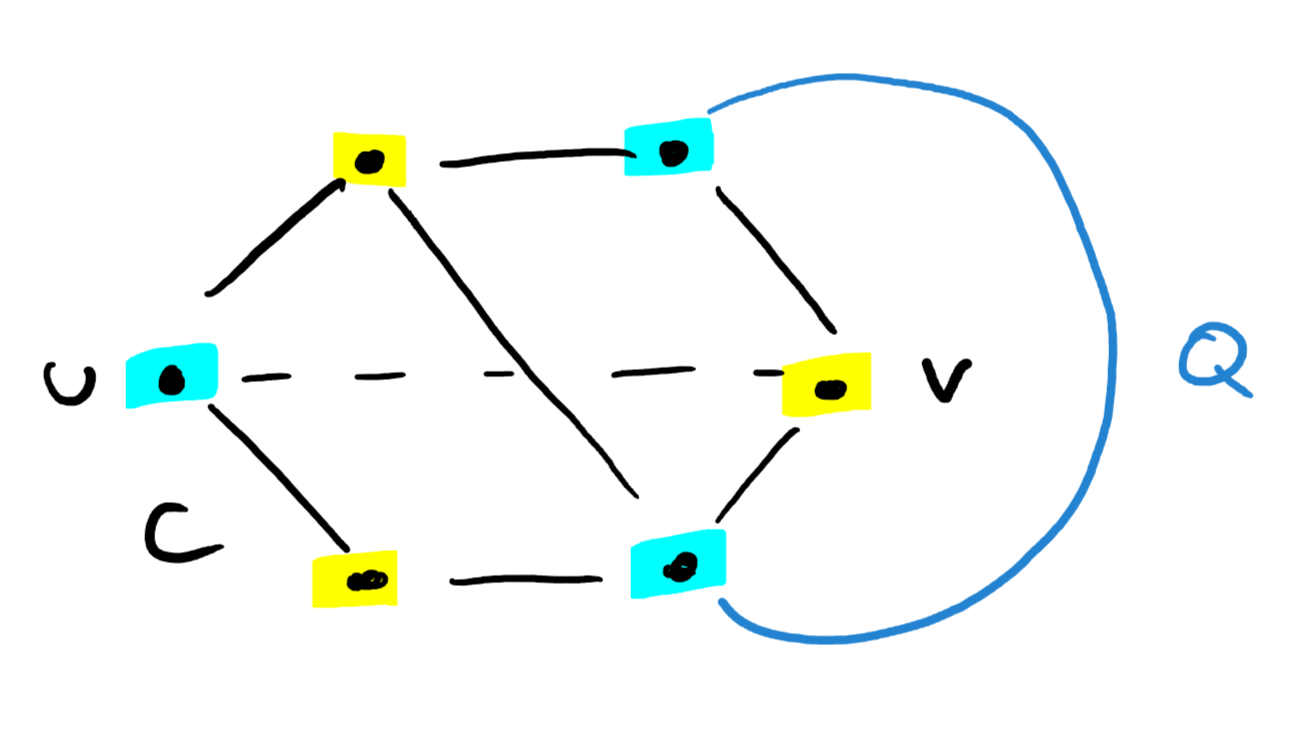
\includegraphics[width=\textwidth]{figures/kuratowski1.png}
            \subcaption{Gegenbeispiel 1}
            \label{fig:kuratowski-bsp1}
        \end{subfigure}
        \begin{subfigure}[c]{\w}
            \centering
            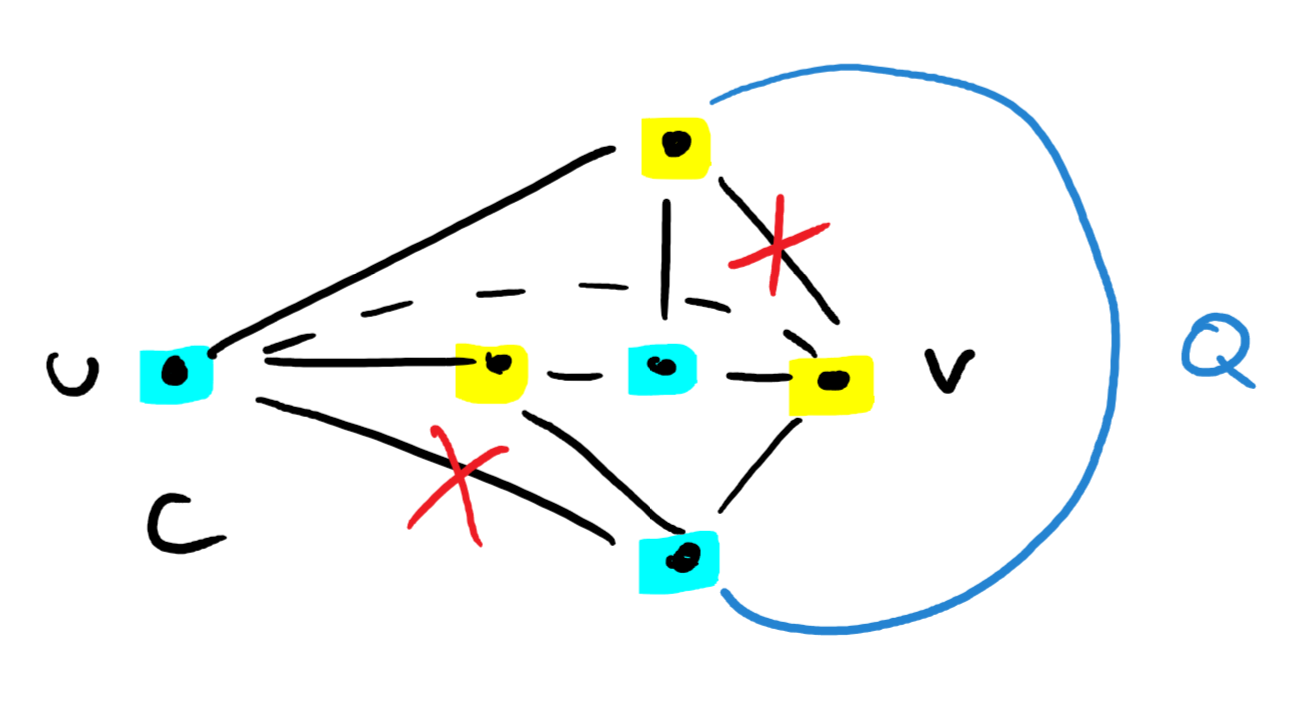
\includegraphics[width=\textwidth]{figures/kuratowski2.png}
            \subcaption{Gegenbeispiel 2}
            \label{fig:kuratowski-bsp2}
        \end{subfigure}
        \begin{subfigure}[c]{\w}
            \centering
            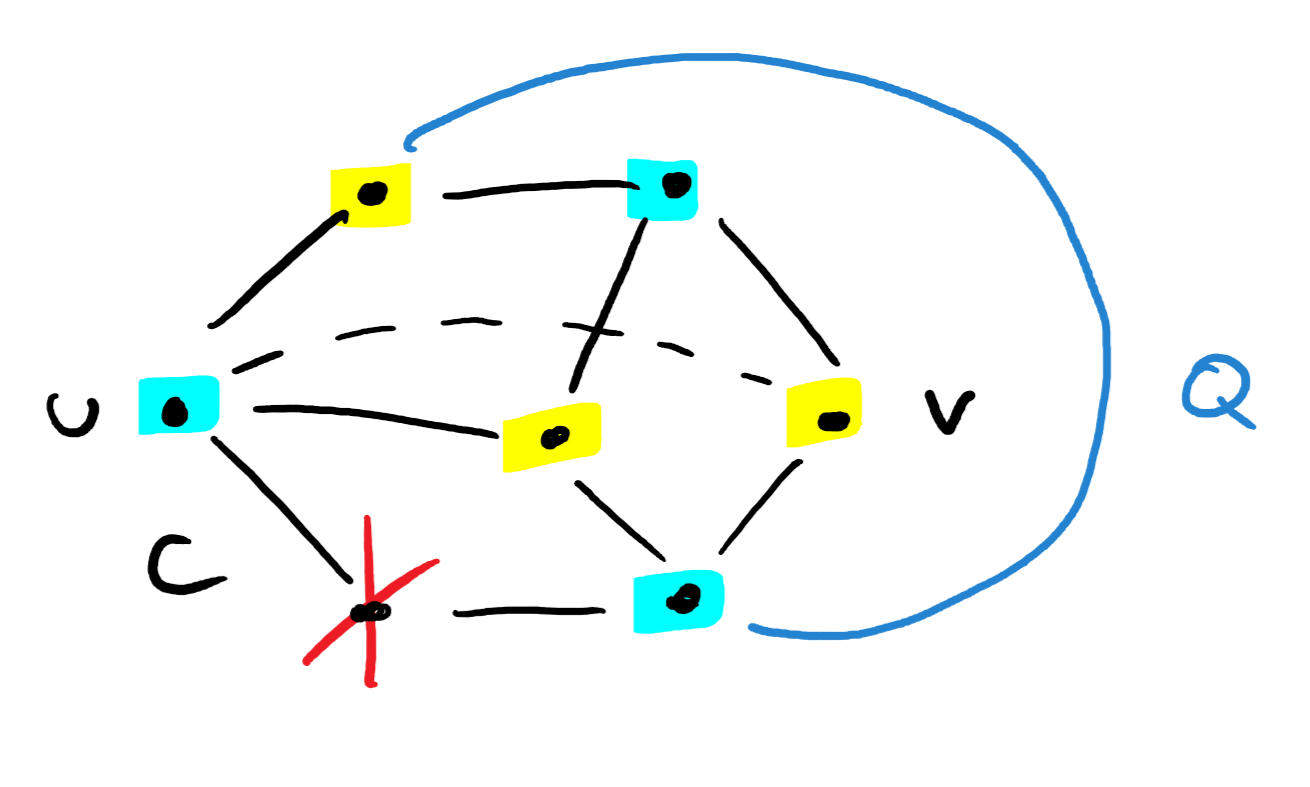
\includegraphics[width=\textwidth]{figures/kuratowski3.png}
            \subcaption{Gegenbeispiel 3}
            \label{fig:kuratowski-bsp3}
        \end{subfigure}
        \begin{subfigure}[c]{\w}
            \centering
            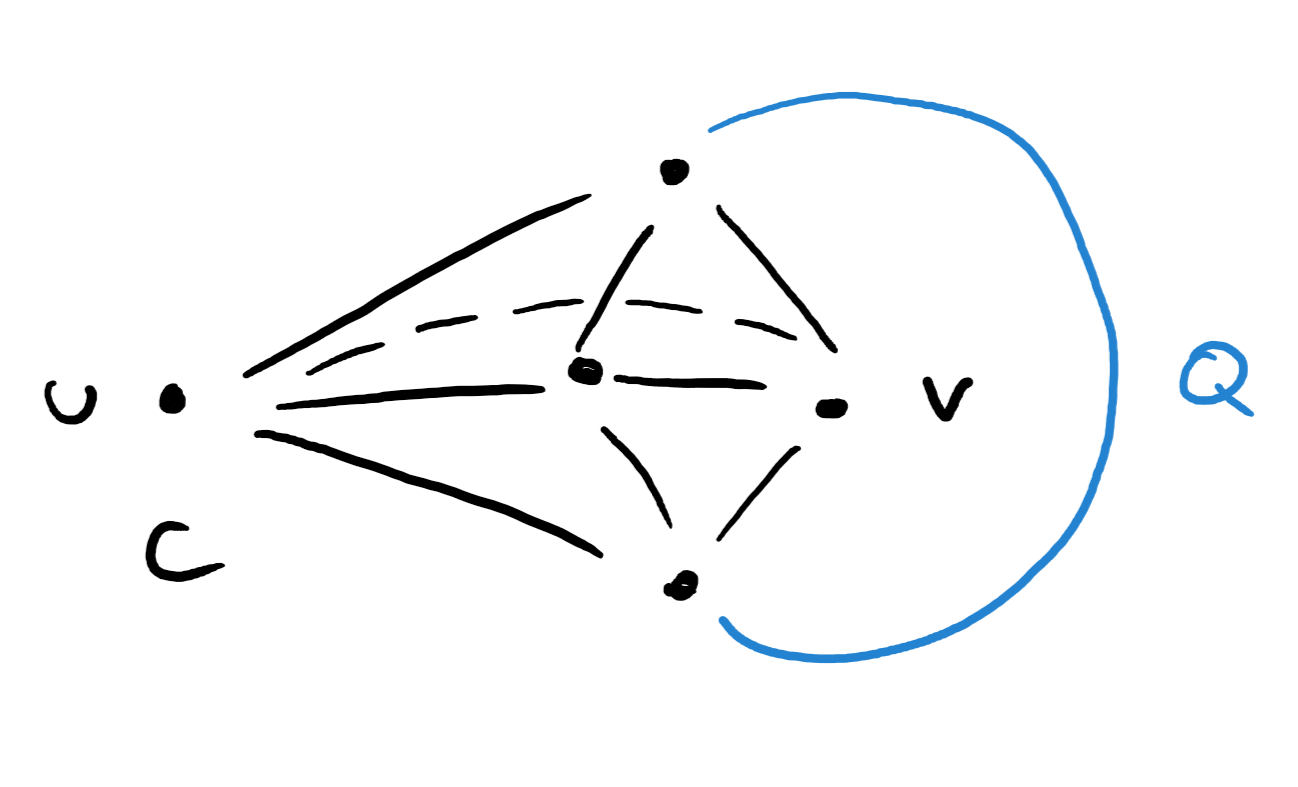
\includegraphics[width=\textwidth]{figures/kuratowski4.png}
            \subcaption{Gegenbeispiel 4}
            \label{fig:kuratowski-bsp4}
        \end{subfigure}
        \caption{Gegenbeispiele für den Beweis von Kuratowskis Theorem}
        \label{fig:kuratowski-bsp}
    \end{figure}
\end{proof}
